\documentclass[../paper.tex]{subfiles}
\begin{document}

\section*{Description}
As discussed in \citep{ComputationalExploration}, in String Theory some basic computational problems are:
\begin{itemize}
    \item Find a probability distribution for all possibilities of (M, V).
    \item For any given (M, V), calculate the resulting spectrum of particles and the interactions between them.
\end{itemize}


There are already existing tools, databases and software available for solving these problems. However, for the current tools, the full problem is to big. This means, better tools should be produced in order to solve these computational problems. In order to explain the situation and how this relates to Scientific Computing, the development of the problem will be shown chronologically.


\section*{Past \& Present}
Software tools, like 'Mathematica', 'Sage' and 'MATLAB', already exist for finding solutions to problems in Mathematics. These tools are not really specific, so for a particular problem, like Riemann-tensors, packages for these tools exist. This sounds good on one hand, but as the "Survival of the Fittest"-theorem from evolutionary biology learns us, the best package should have taken over, but it didn't. This means that there is no such thing as "the best package" yet. All packages have their own pros and cons.

Since there are many mathematical constructs (like groups, manifolds, etc.), there are a lot of representations for these constructs. In order to use all of these constructs effectively together, conversion between these constructs should be possible. The current packages have pro's and cons but there is no package which can handle every single construct effectively together with other constructs. Also, most physicists write their own tools and packages, because this is simply easier than using others'. 

In MATLAB there currently exists a package for a visual simulation on vibrating strings. This function only takes the number of peaks a string has, and outputs this in a animation on how the string would vibrate \ref{Vibrating String}. With an average calculation time of 0.219 for [2,3,4,5] number of peaks, one can see that a lot of computational power is necessary, in order to represent a very high amount of different strings. This is only the first step of the process in proving if 1 of the possible (M,V) shapes contains the Laws of Nature as we know them in our universe. The resulting states of all these strings on the manifold have to be compared to the physics we already know and have to be verified. For example, consider solving a problem with the Finite Element Method, which only solves 1 aspect. These computations already take a lot of time and computational force, the results of the strings and the complete results would take a very long amount of time.

\section*{Future}
In the past, a method has been developed to verify proof and algorithms. The main goal for the future is not only to develop such methods, but also develop the frameworks and theory which make this possible. In new frameworks, researchers would be able to do their work and produce conclusions. These tools should be general for "Mathematical Sciences". As discussed, some software tools are already available. But since there's not a really good package available which can effectively combine constructs together, there are lots of work to be done in this field. Better packages need to be developed. 

Parallel computing might be a good way to deal with the computational types of problems within String Theory. Since constructs sometimes can't work together very well, they might as well process different tasks simultaneously. The results can then be combined. For example, the experimental computation can be done as the first process, while the verification, so calculating that need to be produced in the given situation, can be done as a second process at the same time. However these 2 processes contain different constructs, the results of both can be looked at and verified. This example shows that multiple processes with the complextiy of the String Theory computations can be done at the same time. This saves computation time and thus, more situations can be evaluated in less time. Especially the second part is very important because the amount of possibilities, though finite, is very high. This way of processing might help String Theorists to solve problems faster.

\begin{figure}[h]
\centering
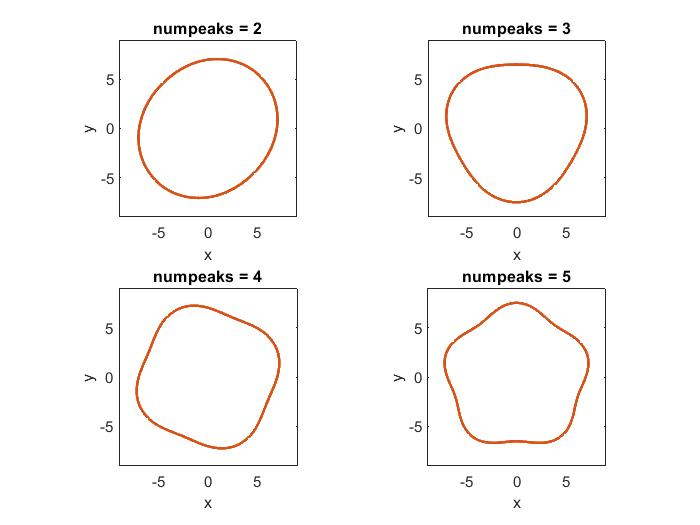
\includegraphics[scale = 0.5]{Computational Problems/vibratingstring.jpg}
\caption{Vibrating String}
\label{Vibrating String}
\end{figure}

\end{document}